\documentclass[../main.tex]{subfiles}

\begin{document}
Una vez realizado el modelado en Protegé, se pueden realizar diversas consultas SPARQL para obtener información tanto de la Base de Datos como de los datos en sí que contiene este modelado. En primer lugar, se mostrarán varias consultas SPARQL que proporcionen información sobre la base de datos. Y, en segundo lugar, se podrán observar otro tipo de consultas extra sobre los datos. \\

Para la realización de estas consultas, ha sido utilizado GraphDB
\subsection{Consula SPARQL 1}
La primera consulta que se va a realizar será la más típica para conocer la base de datos. Lo principal para conocer la base de datos, es saber que clases la compone.
\begin{lstlisting}
PREFIX owl:<http://www.w3.org/2002/07/owl#>
PREFIX rdf: <http://www.w3.org/1999/02/22-rdf-syntax-ns#>
PREFIX rdfs: <http://www.w3.org/2000/01/rdf-schema#>
PREFIX farma: <http://www.semanticweb.org/mruiz/ontologies/2022/10/medicamentos#>

select ?classes where {
    ?classes a owl:Class
}
\end{lstlisting}
Esta consulta proporciona el siguiente resultado:
\begin{figure}[h]
    \centering
    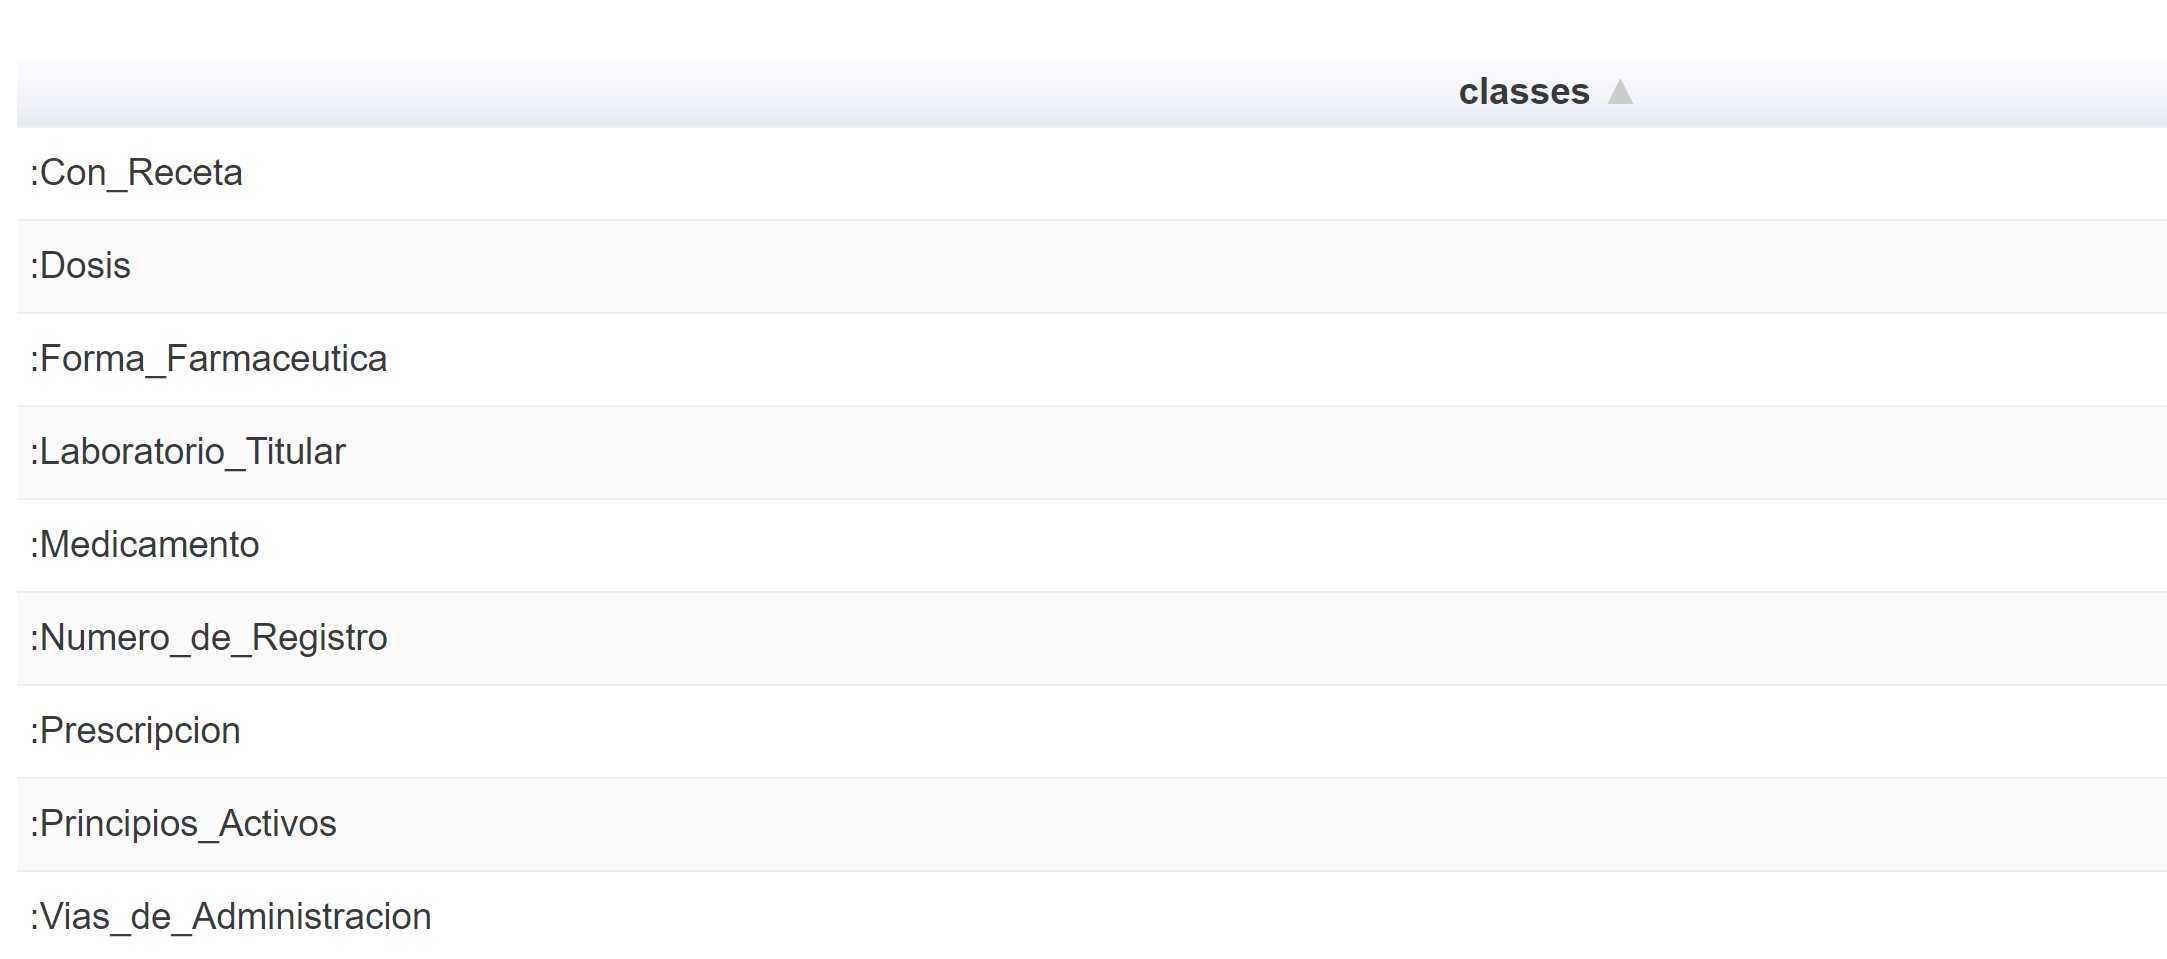
\includegraphics[scale=0.2]{images/clases_sparql.png}
    \caption{Consulta SPARQL 1}
    \label{fig:mesh1}
\end{figure}

\subsection{Consula SPARQL 2}
Otra consulta muy común para conocer el modelo, es obtener las propiedades definidas en este, para ello, se realiza la siguiente consulta:
\begin{lstlisting}
PREFIX owl:<http://www.w3.org/2002/07/owl#>
PREFIX rdf: <http://www.w3.org/1999/02/22-rdf-syntax-ns#>
PREFIX rdfs: <http://www.w3.org/2000/01/rdf-schema#>
PREFIX farma: <http://www.semanticweb.org/mruiz/ontologies/2022/10/medicamentos#>
select ?property
where { 
    {?property rdf:type owl:ObjectProperty . }
    UNION {?property rdf:type owl:DatatypeProperty}
}
\end{lstlisting}

Esta consulta proporciona el siguiente resultado:
\begin{figure}[h]
    \centering
    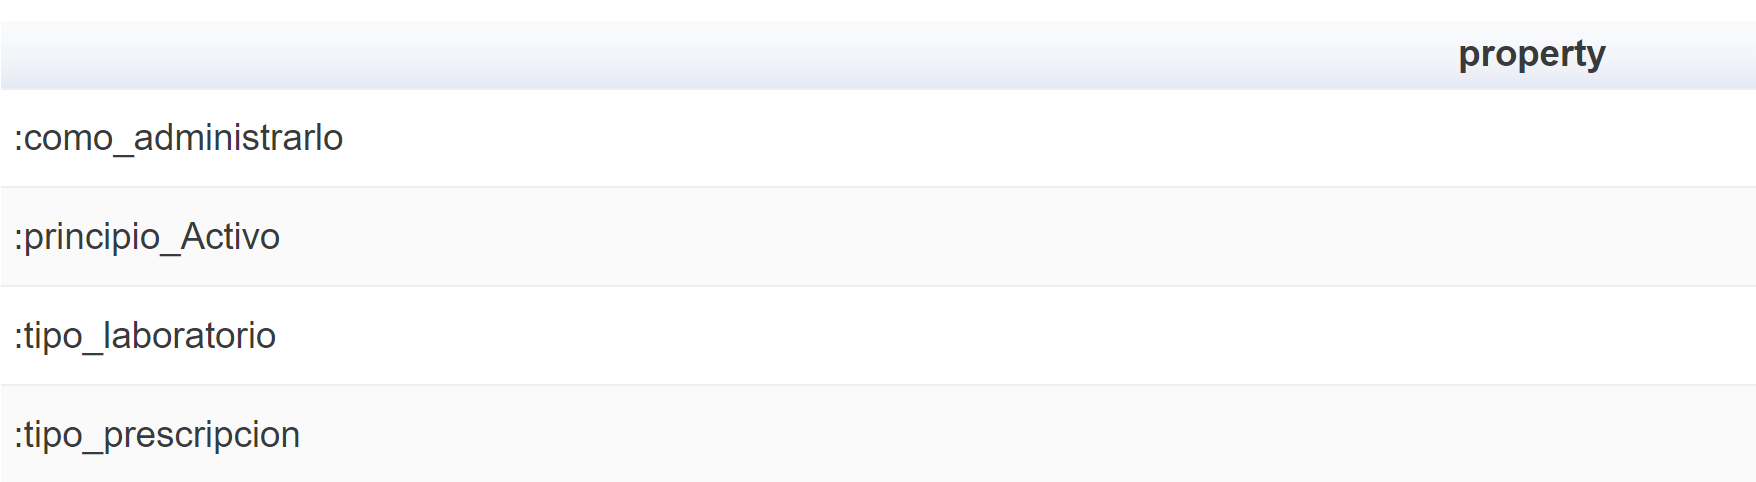
\includegraphics[scale=0.2]{images/propiedades-sparql.png}
    \caption{Consulta SPARQL 2}
    \label{fig:mesh1}
\end{figure}

\subsection{Consula SPARQL 3}
Por último, se mostrarán las clases que tienen una propiedad dada, en este caso la propiedad es "como administrarlo".
La consulta se realiza de la siguiente manera:
\begin{lstlisting}
PREFIX owl:<http://www.w3.org/2002/07/owl#>
PREFIX rdf: <http://www.w3.org/1999/02/22-rdf-syntax-ns#>
PREFIX rdfs: <http://www.w3.org/2000/01/rdf-schema#>
PREFIX farma: <http://www.semanticweb.org/mruiz/ontologies/2022/10/medicamentos#>

select distinct ?class where { 
    ?individuo farma:como_administrarlo ?v . 
    ?individuo rdf:type ?class . 
    
} 
\end{lstlisting}

El resultado es el siguiente:
\begin{figure}[h]
    \centering
    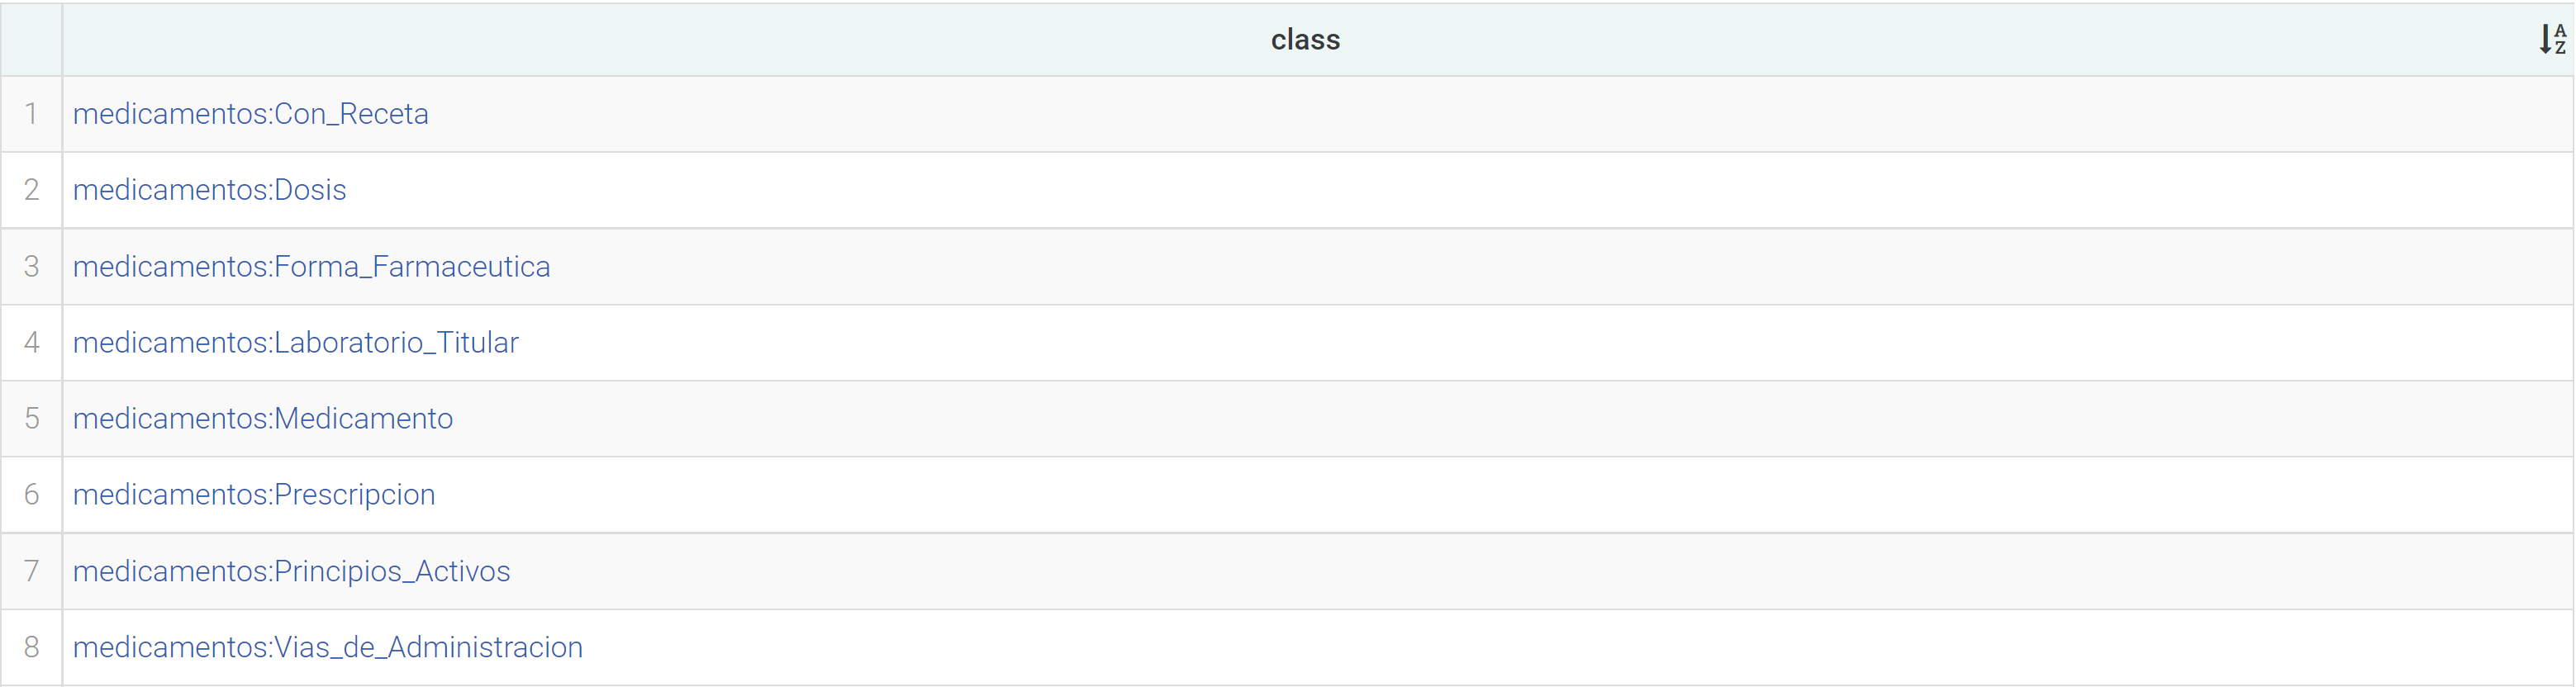
\includegraphics[scale=0.2]{images/comoAdministrarlo.png}
    \caption{Consulta SPARQL 3}
    \label{fig:mesh1}
\end{figure}


Una vez se han realizado las consultas típicas y esenciales para conocer la base de datos. se propcede a la realización de las consultas con los datos proporcionados.

\subsection{Consula SPARQL 4}

En esta consulta, se han buscado todos los medicamentos que necesitan ser adquiridos mediante prescripción médica.

La consulta SPARQL se ha diseñado de la siguiente manera:
\begin{lstlisting}
PREFIX owl:<http://www.w3.org/2002/07/owl#>
PREFIX rdf: <http://www.w3.org/1999/02/22-rdf-syntax-ns#>
PREFIX rdfs: <http://www.w3.org/2000/01/rdf-schema#>
PREFIX farma: <http://www.semanticweb.org/mruiz/ontologies/2022/10/medicamentos#>

select distinct ?medicamento ?conReceta
where {
    ?medicamento farma:como_adquirirlo ?conReceta
	FILTER(?conReceta = "Con receta")   
}
\end{lstlisting}
Esta consulta proporciona el siguiente resultado:
\begin{figure}[h]
    \centering
    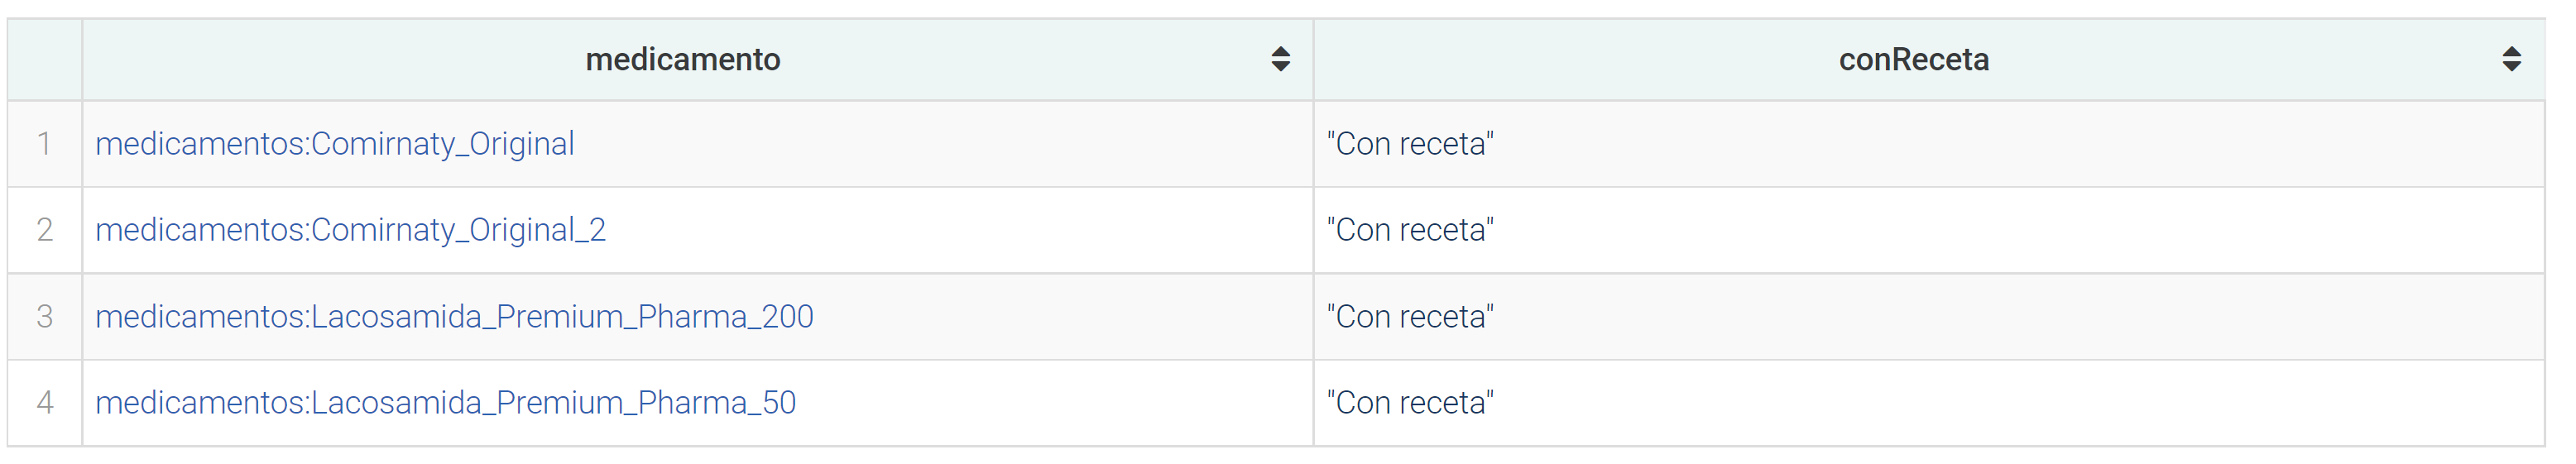
\includegraphics[scale=0.2]{images/medicamentosReceta.png}
    \caption{Consulta SPARQL 4}
    \label{fig:mesh1}
\end{figure}

\subsection{Consula SPARQL 5}
La última consulta, se muestran los medicamentos recubiertos con película junto a sus principios activos.
La consulta SPARQL se ha diseñado de la siguiente forma:
\begin{lstlisting}
PREFIX owl:<http://www.w3.org/2002/07/owl#>
PREFIX rdf: <http://www.w3.org/1999/02/22-rdf-syntax-ns#>
PREFIX rdfs: <http://www.w3.org/2000/01/rdf-schema#>
PREFIX farma: <http://www.semanticweb.org/mruiz/ontologies/2022/10/medicamentos#>

select distinct ?medicamento ?conPelicula ?principioActivo
where {
    ?medicamento farma:principio_Activo ?principioActivo .
    ?medicamento farma:tipos_de_forma_farmaceutica ?conPelicula
	FILTER(?conPelicula = "Comprimido recubierto con pelicula")   
}
\end{lstlisting}
Esta consulta proporciona el siguiente resultado:
\begin{figure}[h]
    \centering
    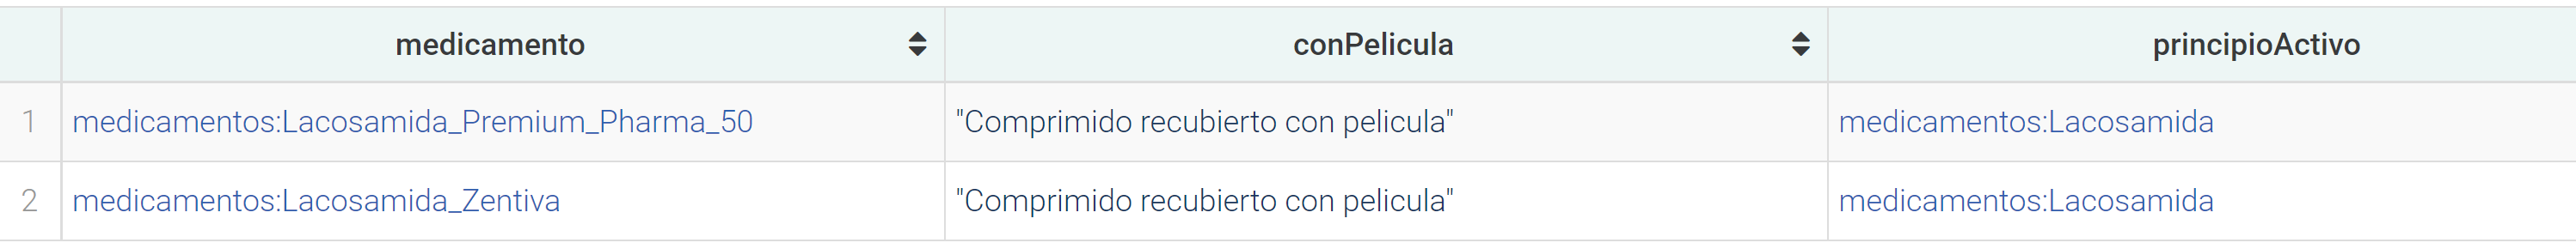
\includegraphics[scale=0.2]{images/conPelicula-SPARQL.png}
    \caption{Consulta SPARQL 5}
    \label{fig:mesh1}
\end{figure}





\end{document}